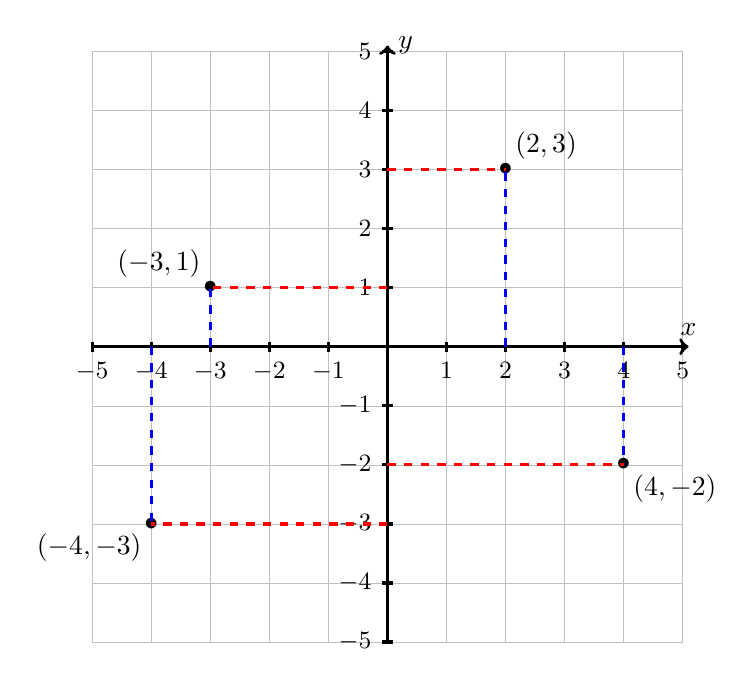
\begin{tikzpicture}[scale=.75]
  \def\xmin{-5}
  \def\xmax{5}
  \def\ymin{-5}
  \def\ymax{5}
  \path [draw, help lines, opacity=.5]  (\xmin,\ymin) grid (\xmax,\ymax);
  \foreach \i in {1,...,5} 
  \draw [very thick] (\i,2.5pt) -- +(0,-5pt) node [anchor=north, font=\small] {$\i$}
  (-\i,2.5pt) -- +(0,-5pt) node [anchor=north, font=\small] {$-\i$} 
  (2.5pt,\i) -- +(-5pt,0) node [anchor=east, font=\small] {$\i$}
  (2.5pt,-\i) -- +(-5pt,0) node [anchor=east, font=\small] {$-\i$};

  \draw [very thick,->] (\xmin,0) -- (\xmax+.1,0) node [anchor=south] {$x$};
  \draw [very thick,->] (0,\ymin) -- (0,\ymax+.1) node [anchor=west] {$y$};

  \node at (2,3) {$\bullet$};
  \node [above right] at (2,3) {$(2,3)$};
  \draw [dashed,color=blue,very thick] (2,0) -- (2,3);
  \draw [dashed,color=red,very thick] (0,3) -- (2,3);

  \node at (-3,1) {$\bullet$};
  \node [above left] at (-3,1) {$(-3,1)$};
  \draw [dashed,color=blue,very thick] (-3,0) -- (-3,1);
  \draw [dashed,color=red,very thick] (0,1) -- (-3,1);

  \node at (-4,-3) {$\bullet$};
  \node [below left] at (-4,-3) {$(-4,-3)$};
  \draw [dashed,color=blue,very thick] (-4,0) -- (-4,-3);
  \draw [dashed,color=red,very thick] (0,-3) -- (-4,-3);

  \node at (4,-2) {$\bullet$};
  \node [below right] at (4,-2) {$(4,-2)$};
  \draw [dashed,color=blue,very thick] (4,0) -- (4,-2);
  \draw [dashed,color=red,very thick] (0,-2) -- (4,-2);
\end{tikzpicture}
